\section{Warm up: Margins}
\label{sec:q1}

\begin{enumerate}

\item ~[5 points] Suppose we want to use an SVM to learn the XOR
  function in two dimensions. We know that XOR is not linearly
  separable, so we apply a feature transformation. In order to do so,
  we map the input $[x_1, x_2] $ into a space consisting of two
  features: $x_1$ and $x_1 x_2$. All examples are Boolean (1 for
  positive and -1 for negative) What is the maximal margin? Draw the
  separating line back in original Euclidean input space.

  \begin{table}[H]
    \centering
    \begin{tabular}{| c | c | c  |  c | }
      \hline
      $x_1$ & $x_2$  & $x_1x_2$ & $Label$ \\
      \hline
      $-1$ & $-1$ & $+1$ & $-1$\\
      $-1$ & $+1$ & $-1$ & $+1$\\
      $+1$ & $-1$ & $-1$ & $+1$\\
      $+1$ & $+1$ & $+1$ & $-1$\\
      \hline
    \end{tabular}
    \caption*{XOR Function truth table}
  \end{table}

The XOR function truth table shows the original inputs $x_1$ and $x_2$ along with the new feature $x1x2$. The label column shows $x_1 \oplus x_2$. Figure \ref{XorSvm} shows the new space with features $x_1$ and $x_1x_2$. The points in this input space are shown along with their labels. The axis for the feature $x_1$ is the linear separator with the maximum margin and is shown as the bold line. The four features in the new space become support vectors and the margin is half the distance between the lines joining the support vectors.

The input features $x_1$ and $x_2$ in the original feature space are shown in figure \ref{XorOriginal}. The lines joining the support vectors now intersect each other. The line of maximum margin in figure \ref{XorSvm} was the one where $x_1$ varied from $+\infty$ to $+\infty$ and $x_1x_2$ was $0$. The corresponding line in the original feature space would be the one where $x_1$ varies from $+\infty$ to $+\infty$ and $x_2$ is $0$, as $x_2=0$ corresponds to the case where $x_1x_2=0$ in the new feature space. This line of maximum separation is shown in bold in figure \ref{XorOriginal}.
  \begin{figure}[H]
    \centering
    \begin{tikzpicture}[domain=0:2]
      \draw[<->] (-3.2,0) -- (3.2,0) node[below right] {$x_1$};
      \draw[<->] (0,-4) -- (0,4) node[left] {$x_1x_2$};
      \draw [<->] (-3.2,3) -- (3.2,3) ;
      \draw [<->] (-3.2,-3) -- (3.2,-3) ;
      \draw [ultra thick] (-3.2,0) -- (3.2,0) ;
      \foreach \Point/\PointLabel in {(-3,3)/, (-3,-3)/, (3,-3)/, (3,3)/}
\draw[fill=black] \Point circle (0.05) node[above right] {$\PointLabel$};
\node [above] at (-3,  3) {$(-1, +1)$};
\node [below] at (-3,  3) {$ -1$};
\node [above] at (-3,  -3) {$(-1, -1)$};
\node [below] at (-3,  -3) {$ +1$};
\node [above] at (3,  -3) {$(+1, -1)$};
\node [below] at (3,  -3) {$ +1$};
\node [above] at (3,  3) {$(+1, +1)$};
\node [below] at (3,  3) {$ -1$};
    \end{tikzpicture}
    \caption{Separation of XOR function in feature space $x_1$ and $x_1x_2$.} \label{XorSvm}
  \end{figure}

  \begin{figure}[H]
    \centering
    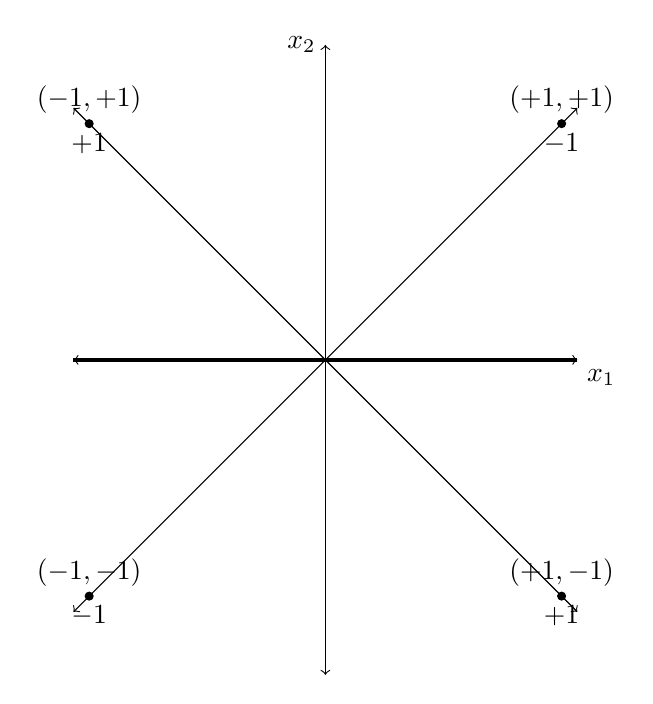
\begin{tikzpicture}[domain=0:2]
      \draw[<->] (-3.2,0) -- (3.2,0) node[below right] {$x_1$};
      \draw[<->] (0,-4) -- (0,4) node[left] {$x_2$};
      \draw [<->] (-3.2,-3.2) -- (3.2,3.2) ;
      \draw [<->] (-3.2,3.2) -- (3.2,-3.2) ;
      \draw [ultra thick] (-3.2,0) -- (3.2,0) ;
      \foreach \Point/\PointLabel in {(-3,3)/, (-3,-3)/, (3,-3)/, (3,3)/}
\draw[fill=black] \Point circle (0.05) node[above right] {$\PointLabel$};
\node [above] at (-3,  3) {$(-1, +1)$};
\node [below] at (-3,  3) {$ +1$};
\node [above] at (-3,  -3) {$(-1, -1)$};
\node [below] at (-3,  -3) {$ -1$};
\node [above] at (3,  -3) {$(+1, -1)$};
\node [below] at (3,  -3) {$ +1$};
\node [above] at (3,  3) {$(+1, +1)$};
\node [below] at (3,  3) {$ -1$};
    \end{tikzpicture}
    \caption{Separation of XOR function in original feature space $x_1$ and $x_2$.} \label{XorOriginal}
  \end{figure}
  
\item ~[10 points]  Consider the following collection of points:
  \begin{table}[H]
    \centering
    \begin{tabular}{| c | c | c  ||  c | c | c |}
      \hline
      Point & coordinate  & label & Point & coordinate  & label \\
      \hline
      $x_1$ & (0, 0)             & + & $x_5$ & (0, 1)                                & - \\
      $x_2$ & (1, 0)             & + & $x_6$ & ($\frac{1}{2}$, $\frac{\sqrt{3}}{2}$) & - \\
      $x_3$ & (1, 1)             & + & $x_7$ & ($\frac{3}{2}$, 0)                    & - \\
      $x_4$ & ($\frac{1}{2}$, 0) & + & $x_8$ & (1, $\frac{1}{2}$)                    & - \\
      \hline
    \end{tabular}
    \caption{A collection of points}
  \end{table}

  Suppose we have three training sets comprising of subsets of these
  points. We have
  $$D_1 = \{x_1, x_2, x_3, x_4, x_7\}$$
  $$D_2 = \{x_1, x_5, x_6, x_8\}$$
  $$D_3 = \{x_3, x_4, x_5, x_ 7\}$$

  \begin{enumerate}
  \item ~[6 points] Give the maximum possible margin for $D_1$, $D_2$
    and $D_3$.
  \item ~[2 points] What is the Perceptron mistake bound for these
    dataset. Which has the greatest Perceptron mistake bound.
  \item ~[2 points] Rank the datasets in terms of ``ease of
    learning''. Justify your answer.
  \end{enumerate}

\end{enumerate}


%%% Local Variables:
%%% mode: latex
%%% TeX-master: "hw"
%%% End:
